\documentclass[pdf]{beamer}

\usetheme{CambridgeUS}
\usepackage[utf8x]{inputenc}
\usepackage{listings}
\lstset{basicstyle={\footnotesize}}
\usepackage{graphicx}

\mode<presentation>{}
\title{Building an LLVM Backend}
\subtitle{LLVM 2014 tutorial}
\author{Fraser Cormak \\ Pierre-Andre Saulais \\ Codeplay Software \\ @codeplaysoft}

\begin{document}

%%%%%%%%%%%%%%%%%%%%%%%%%%%%%%%%%%%%%%%%%%%%%%%%%%%%%%%%%%%%%%%%%%%%%%%%%%%%%%%%

\begin{frame}
\titlepage
\end{frame}

%%%%%%%%%%%%%%%%%%%%%%%%%%%%%%%%%%%%%%%%%%%%%%%%%%%%%%%%%%%%%%%%%%%%%%%%%%%%%%%%

\begin{frame}{Introduction}

\begin{itemize}
    \item Yet another talk about creating a LLVM target?
    \item LLVM backend crash course, for beginners
    \begin{itemize}
        \item How-tos and tips
        \item Solution to common problems
    \end{itemize}  
    \item Example target created for this tutorial
    \begin{itemize}
        \item Can be used to see how LLVM works
        \item Can be used as a skeleton to bootstrap new target
    \end{itemize}
\end{itemize}

\end{frame}

%%%%%%%%%%%%%%%%%%%%%%%%%%%%%%%%%%%%%%%%%%%%%%%%%%%%%%%%%%%%%%%%%%%%%%%%%%%%%%%%

\begin{frame}{Overview}

\begin{itemize}
    \item Part 1: Background
    \item Part 2: Creating your own target
    \item Part 3: How-tos for specific tasks
    \item Part 4: Troubleshooting and tips
\end{itemize}

\end{frame}

%%%%%%%%%%%%%%%%%%%%%%%%%%%%%%%%%%%%%%%%%%%%%%%%%%%%%%%%%%%%%%%%%%%%%%%%%%%%%%%%

%%%%%%%%%%%%%%%%%%%%%%%%%%%%%%%%%%%%%%%%%%%%%%%%%%%%%%%%%%%%%%%%%%%%%%%%%%%%%%%%

\talksection{What \& why: LLVM}

\begin{frame}{What is LLVM?}

\begin{itemize}
    \item Collection of modular compiler and toolchain technologies
    \item Started as a research project
    \item Apple took it on in 2005
    \item Grown to include many sub-projects:
    \begin{itemize}
      \item LLVM Core - Optimizers, code generators
      \item Clang     - C/C++/Objective-C front-end
      \item LLDB      - Debugger
      \item libc++    - Conformant \& performant C++ STL
      \item lld       - System linker
    \end{itemize}
\end{itemize}

\end{frame}

%%%%%%%%%%%%%%%%%%%%%%%%%%%%%%%%%%%%%%%%%%%%%%%%%%%%%%%%%%%%%%%%%%%%%%%%%%%%%%%%

\begin{frame}{Why LLVM?}

\begin{itemize}
    \item Open source
    \item Nice, permissive license
    \item Modular
    \item Active community
\end{itemize}

\end{frame}

%%%%%%%%%%%%%%%%%%%%%%%%%%%%%%%%%%%%%%%%%%%%%%%%%%%%%%%%%%%%%%%%%%%%%%%%%%%%%%%%

\talksection{Our backend: LEG}

\begin{frame}{Example target: LEG}

\begin{itemize}
    \item Simple, RISC-like architecture
    \begin{itemize}
        \item Very small subset of ARM
    \end{itemize}
    \item 12 integer registers (32-bit)
    \begin{itemize}
        \item r0, r1, ..., r9, sp (stack pointer), lr (return address)
    \end{itemize}
    \item Instructions:
    \begin{itemize}
        \item 32-bit arithmetic (add, subtract, multiply, mad)
        \item 32-bit register move, 16-bit constant moves
        \item load, store, branch, branch and link
    \end{itemize}
\end{itemize}

\end{frame}

%%%%%%%%%%%%%%%%%%%%%%%%%%%%%%%%%%%%%%%%%%%%%%%%%%%%%%%%%%%%%%%%%%%%%%%%%%%%%%%%

\begin{frame}[fragile]{LEG assembly examples}

\begin{itemize}
    \item Function that adds two integers
    \begin{itemize}
        \item The arguments are passed in registers: \texttt{a} in \texttt{r0}, \texttt{b} in \texttt{r1}
        \item The return value is stored in \texttt{r0}
    \end{itemize}
    \item Returns to the caller using \texttt{b}
    \begin{itemize}
        \item \texttt{lr} contains the function's return address
    \end{itemize}
\end{itemize}

\begin{codebox}
int foo(int a, int b) {
    int result = a + b;   // r0 + r1
    return result;        // r0
}
\end{codebox}
\codecaption{ex1.c}

\begin{codebox}
.foo:
    add r0, r0, r1
    b lr
\end{codebox}
\codecaption{ex1.s}

\end{frame}

%%%%%%%%%%%%%%%%%%%%%%%%%%%%%%%%%%%%%%%%%%%%%%%%%%%%%%%%%%%%%%%%%%%%%%%%%%%%%%%%

\begin{frame}[fragile]{LEG assembly examples}

\begin{itemize}
    \item Function that either adds or subtracts two integers
    \item The result depends on which argument is greater
    \begin{itemize}
        \item \texttt{cmp} compares the arguments
        \item \texttt{b} branches to the '\texttt{if\_else}' basic block, using:
        \begin{itemize}
            \item The '\texttt{le}' predicate
            \item The implicit condition flag register set by \texttt{cmp}
        \end{itemize}
        \item Fall-through to '\texttt{if\_then}' if the predicate doesn't match
    \end{itemize}
\end{itemize}

\begin{minipage}[t]{0.50\linewidth}
\begin{codebox}
int ex6(int a, int b) {
    if (a > b) {
        return a + b;
    } else {
        return a - b;
    }
}


\end{codebox}
\codecaption{ex6.c}
\end{minipage}
\begin{minipage}[t]{0.49\linewidth}
\begin{codebox}
.ex6:
    cmp r0, r1
    ble .if_else
.if_then:
    add r0, r0, r1
    bx lr
.if_else:
    sub r0, r0, r1
    bx lr
\end{codebox}
\codecaption{ex6.s}
\end{minipage}

\end{frame}

%%%%%%%%%%%%%%%%%%%%%%%%%%%%%%%%%%%%%%%%%%%%%%%%%%%%%%%%%%%%%%%%%%%%%%%%%%%%%%%%

\talksection{LLVM Backend: The big picture}

\begin{frame}{LLVM Backend: The big picture}

\begin{itemize}
    \item Pipeline structure
    \begin{itemize}
        \item Transforms your program many times using different stages
        \item Starts target-independent, then gets increasingly target-specific
    \end{itemize}
    \item Different representations are used
    \begin{itemize}
        \item Tells you roughly where you are in the pipeline
        \item Different instruction namespaces
    \end{itemize}
    \item Check it out (IR and MI representations only):
    \begin{itemize}
        \item \texttt{llc foo.ll -print-after-all 2>\&1 > foo.log}
    \end{itemize}
\end{itemize}

\pipelinemap{IR → SelectionDAG → MachineDAG → MachineInstr → MCInst}{15.5ex}

\end{frame}

%%%%%%%%%%%%%%%%%%%%%%%%%%%%%%%%%%%%%%%%%%%%%%%%%%%%%%%%%%%%%%%%%%%%%%%%%%%%%%%%

\begin{frame}[fragile]{A look at an IR module}

\begin{itemize}
    \item Linear representation
    \begin{itemize}
        \item Basic blocks are lists of instructions
        \item Control Flow Graph (CFG) of basic blocks
    \end{itemize}
    \item High-level, target-agnostic
    \begin{itemize}
        \item Exceptions: data layout, triple, intrinsics
    \end{itemize}
    \item Most instructions define values
    \begin{itemize}
        \item Typed (e.g. \texttt{i32}, \texttt{float}, \texttt{<4 x i32>})
        \item Defined once (SSA), no registers
    \end{itemize}
\end{itemize}

\begin{codebox}
target datalayout = "e-m:e-p:32:32-i1:8:32-i8:8:32-i16:16:32-i64:32-f64-..."
target triple = "leg"

define i32 @foo(i32 %a, i32 %b) {
    %c = add i32 %a, %b
    ret i32 %c
}
\end{codebox}
\codecaption{ex1b.ll}

\pipelinemap{\codeempha{IR} → SelectionDAG → MachineDAG → MachineInstr → MCInst}{0.0ex}

\end{frame}

%%%%%%%%%%%%%%%%%%%%%%%%%%%%%%%%%%%%%%%%%%%%%%%%%%%%%%%%%%%%%%%%%%%%%%%%%%%%%%%%

\begin{frame}{A look at a SelectionDAG graph}

\begin{minipage}[t]{0.50\linewidth}
    \begin{itemize}
        \item Graph representation
        \item Operations as nodes
        \begin{itemize}
            \item Mostly target-agnostic
            \begin{itemize}
                \item Semantics defined by LLVM
                \item ISD namespace for opcodes
            \end{itemize}
            \item Produce typed value(s)
        \end{itemize}
        \item Dependencies as edges
        \begin{itemize}
            \item Data
            \item \codeemphb{Order ("chain")}
            \item \codeempha{Scheduling ("glue")}
        \end{itemize}
    \end{itemize}
\end{minipage}
\begin{minipage}[t]{0.49\linewidth}
    \begin{figure}
        \vspace{-2.2ex}
        \includegraphics[width = 1.0\textwidth]{examples/ex1b/ex1b-pre-isel.pdf}
    \end{figure}
\end{minipage}

\pipelinemap{IR → \codeempha{SelectionDAG} → MachineDAG → MachineInstr → MCInst}{7.9ex}

\end{frame}

%%%%%%%%%%%%%%%%%%%%%%%%%%%%%%%%%%%%%%%%%%%%%%%%%%%%%%%%%%%%%%%%%%%%%%%%%%%%%%%%

\begin{frame}{A look at a MachineDAG graph}

\begin{minipage}[t]{0.50\linewidth}
    \begin{itemize}
        \item Very similar to SelectionDAG
        \item Target instructions as nodes
        \begin{itemize}
            \item Result of instruction selection
            \item LEG namespace
        \end{itemize}
        \item Similar dependencies
        \item Similar types
    \end{itemize}
\end{minipage}
\begin{minipage}[t]{0.49\linewidth}
    \begin{figure}
        \vspace{-2.2ex}
        \includegraphics[width = 1.00\textwidth]{examples/ex1b/ex1b-post-isel.pdf}
    \end{figure}
\end{minipage}

\pipelinemap{IR → SelectionDAG → \codeempha{MachineDAG} → MachineInstr → MCInst}{3ex}

\end{frame}

%%%%%%%%%%%%%%%%%%%%%%%%%%%%%%%%%%%%%%%%%%%%%%%%%%%%%%%%%%%%%%%%%%%%%%%%%%%%%%%%

\begin{frame}{Before and after instruction selection}

\begin{minipage}[t]{0.50\linewidth}
    Before:
    \begin{figure}
        \vspace{-3.0ex}
        \includegraphics[width = 1.00\textwidth]{examples/ex1b/ex1b-pre-isel.pdf}
    \end{figure}
\end{minipage}
\begin{minipage}[t]{0.49\linewidth}
    After:
    \begin{figure}
        \vspace{-3.0ex}
        \includegraphics[width = 1.00\textwidth]{examples/ex1b/ex1b-post-isel.pdf}
    \end{figure}
\end{minipage}

\pipelinemap{IR → \codeempha{SelectionDAG} → \codeempha{MachineDAG} → MachineInstr → MCInst}{1.7ex}

\end{frame}

%%%%%%%%%%%%%%%%%%%%%%%%%%%%%%%%%%%%%%%%%%%%%%%%%%%%%%%%%%%%%%%%%%%%%%%%%%%%%%%%

\begin{frame}{A look at a MachineInstr block}

\begin{itemize}
    \item Untyped, uses register classes instead
    \begin{itemize}
        \item Virtual registers (before register allocation)
        \item Machine registers (after RA)
    \end{itemize}
    \item Target-specific instructions (LEG namespace)
    \begin{itemize}
        \item Few exceptions (TargetOpcode namespace)
    \end{itemize}
    \item Instruction operands have flags:
    \begin{itemize}
        \item Def for outputs, use for inputs
        \item Kill: last use of a value stored in a register
    \end{itemize}
\end{itemize}

\examplebox{ex1/ex1-mi.txt}

\pipelinemap{IR → SelectionDAG → MachineDAG → \codeempha{MachineInstr} → MCInst}{1.3ex}

\end{frame}

%%%%%%%%%%%%%%%%%%%%%%%%%%%%%%%%%%%%%%%%%%%%%%%%%%%%%%%%%%%%%%%%%%%%%%%%%%%%%%%%

\begin{frame}{Bits of your ISA you need to describe}

\begin{itemize}
    \item Target machine
    \begin{itemize}
        \item Registers, register classes
        \item Calling conventions
    \end{itemize}
    \item Instruction set
    \begin{itemize}
        \item Operands and patterns
        \item Assembly printing and/or instruction encoding
        \item Schedule (not part of this talk)
    \end{itemize}
    \item ...
\end{itemize}

\end{frame}

%%%%%%%%%%%%%%%%%%%%%%%%%%%%%%%%%%%%%%%%%%%%%%%%%%%%%%%%%%%%%%%%%%%%%%%%%%%%%%%%

\talksection{Describing the target machine}

\begin{frame}{TableGen}

\begin{itemize}
    \item C++-style syntax
    \item Different set of backends
    \begin{itemize}
        \item RegisterInfo, InstrInfo, AsmWriter, ...
    \end{itemize}
    \item TableGen backends generate .inc files
    \begin{itemize}
        \item Included by your C++ files
    \end{itemize}
    \item More information:
    \begin{itemize}
        \item \url{llvm.org/docs/TableGen/index.html}
        \item \url{llvm.org/docs/TableGen/BackEnds.html}
    \end{itemize}
\end{itemize}

\end{frame}

%%%%%%%%%%%%%%%%%%%%%%%%%%%%%%%%%%%%%%%%%%%%%%%%%%%%%%%%%%%%%%%%%%%%%%%%%%%%%%%%

\begin{frame}[fragile]{Describing registers with TableGen}

\begin{itemize}
    \item TableGen provides the 'Register' class
    \begin{itemize}
        \item Can use the 'HWEncoding' field for encodings
    \end{itemize}
    \item Referenced as “LEG::R0” in C++
\end{itemize}

\begin{codebox}
class LEGReg<bits<16> Enc, string n> : Register<n> {
  Let HWEncoding = Enc;
  let Namespace = "LEG";
}

def R0 : LEGReg< 0, "r0" >;
...
def SP : LEGReg< 10, "sp" >;
\end{codebox}
\codecaption{LEGRegisterInfo.td}

\end{frame}

%%%%%%%%%%%%%%%%%%%%%%%%%%%%%%%%%%%%%%%%%%%%%%%%%%%%%%%%%%%%%%%%%%%%%%%%%%%%%%%%

\begin{frame}[fragile]{Describing registers with TableGen}

\begin{itemize}
    \item Can automate trivial definitions
\end{itemize}

\begin{codebox}
foreach i = 0-9 in {
  def R#i : R<i, "r"#i>;
}
\end{codebox}
\codecaption{LEGRegisterInfo.td}

\begin{itemize}
    \item Group registers into register classes
\end{itemize}

\begin{codebox}
def GRRegs : RegisterClass<"LEG", [i32], 32,
  (add SP, (sequence "R%i", 0, 9))>;
\end{codebox}
\codecaption{LEGRegisterInfo.td}

\end{frame}

%%%%%%%%%%%%%%%%%%%%%%%%%%%%%%%%%%%%%%%%%%%%%%%%%%%%%%%%%%%%%%%%%%%%%%%%%%%%%%%%

\talksection{Describing the instruction set}

\begin{frame}{Describing instructions: Overview}

\begin{itemize}
    \item Let's start with a simple instruction: \texttt{ADDrr}
    \begin{itemize}
        \item Adds two registers together
    \end{itemize}
    \item We define it in lib/Target/LEG/LEGInstrInfo.td
    \item What we need to specify:
    \begin{itemize}
        \item Operands
        \item Assembly string
        \item Instruction pattern
    \end{itemize}
\end{itemize}

\end{frame}

%%%%%%%%%%%%%%%%%%%%%%%%%%%%%%%%%%%%%%%%%%%%%%%%%%%%%%%%%%%%%%%%%%%%%%%%%%%%%%%%

\begin{frame}[fragile]{Describing instructions: Operands}

\begin{itemize}
    \item List of definitions or outputs ('outs')
    \item List of uses or inputs ('ins')
    \item Operand class:
    \begin{itemize}
        \item Register class (e.g. GRRegs)
        \item Immediate (e.g. i32imm)
        \item More complex operands (e.g. reg + imm for load/store)
    \end{itemize}
\end{itemize}

\begin{codebox}[commandchars=\\\{\}]
def ADDrr : InstLEG<\codeempha{(outs GRRegs:$dst)},
                    \codeempha{(ins GRRegs:$src1, GRRegs:$src2)},
                    "add $dst, $src1, $src2",
                    [(set i32:$dst, (add i32:$src1, i32:$src2))]>;
\end{codebox}
\codecaption[-10.2ex]{LEGInstrInfo.td}

\vspace{5ex}
\begin{itemize}
    \item Result:
\end{itemize}
\examplebox[firstline=4,lastline=4,gobble=1]{ex1/ex1-mi.txt}

\end{frame}

%%%%%%%%%%%%%%%%%%%%%%%%%%%%%%%%%%%%%%%%%%%%%%%%%%%%%%%%%%%%%%%%%%%%%%%%%%%%%%%%

\begin{frame}[fragile]{Describing instructions: Selection Patterns}

\begin{itemize}
    \item Matches nodes in the SelectionDAG
    \begin{itemize}
        \item Nodes get turned into MachineInstrs during ISel
        \item If pattern is omitted, selection needs to be done in C++
    \end{itemize}
    \item Syntax:
    \begin{itemize}
        \item One pair of parenthesis defines one node
        \item Nodes have DAG operands, with 'MVT' type (e.g. i32)
        \item Map DAG operands to MI operands
    \end{itemize}
\end{itemize}

\begin{codebox}[commandchars=\\\{\}]
def ADDrr : InstLEG<(outs GRRegs:$dst),
                    (ins GRRegs:$src1, GRRegs:$src2),
                    "add $dst, $src1, $src2",
                    \codeempha{[(set i32:$dst, (add i32:$src1, i32:$src2))]}>;
\end{codebox}
\codecaption[-10.2ex]{LEGInstrInfo.td}

\vspace{5ex}
\begin{itemize}
    \item Result:
\end{itemize}
\examplebox[firstline=4,lastline=4,gobble=1]{ex1/ex1-mi.txt}

\end{frame}

%%%%%%%%%%%%%%%%%%%%%%%%%%%%%%%%%%%%%%%%%%%%%%%%%%%%%%%%%%%%%%%%%%%%%%%%%%%%%%%%

\begin{frame}[fragile]{Constants}

\begin{itemize}
    \item Using constants in IR produces errors at this point
    \item We need to specify how to generate ('materialize') constants
    \item For example, with a 'move' instruction
    \begin{itemize}
        \item E.g. MOVLO for 16-bit constants
    \end{itemize}
\end{itemize}

\begin{itemize}
    \item Example:
\end{itemize}
\examplebox[firstline=8,lastline=8,gobble=4]{ex2/ex2.ll}

\begin{itemize}
    \item Result:
\end{itemize}
\begin{codebox}
LLVM ERROR: Cannot select: 0x29d4350: i32 = Constant<2> [ID=2]
In function: main
\end{codebox}

\end{frame}

%%%%%%%%%%%%%%%%%%%%%%%%%%%%%%%%%%%%%%%%%%%%%%%%%%%%%%%%%%%%%%%%%%%%%%%%%%%%%%%%

\begin{frame}[fragile]{Constants}

\begin{itemize}
    \item Let's define this move instruction:
\end{itemize}

\begin{codebox}
def MOVLOi16 : InstLEG<(outs GRRegs:$dst),
                      (ins i32imm:$src),
                      "movw $dst, $src",
                      [(set i32:$dst, i32imm:$src)]> {
  let isMoveImm = 1;
}
\end{codebox}
\codecaption{LEGInstrInfo.td}

\begin{itemize}
    \item Example:
\end{itemize}
\examplebox[firstline=8,lastline=8,gobble=4]{ex2/ex2.ll}

\begin{itemize}
    \item Result:
\end{itemize}
\examplebox[firstline=6,lastline=7,gobble=1]{ex2/ex2-ADDrr-MOVLO-mi.txt}

\end{frame}

%%%%%%%%%%%%%%%%%%%%%%%%%%%%%%%%%%%%%%%%%%%%%%%%%%%%%%%%%%%%%%%%%%%%%%%%%%%%%%%%

\begin{frame}[fragile]{Constants}

\begin{itemize}
    \item What if the instruction accepts an immediate operand?
\end{itemize}

\begin{codebox}[commandchars=\\¬|]
def \codeempha¬LEGimm8| : Operand<i32>, ImmLeaf<i32, [{
  return Imm >= 0 && Imm < 256;
}]>;

def ADDri : InstLEG<(outs GRRegs:$dst),
                    (ins GRRegs:$src1, \codeempha¬i32imm|:$src2),
                    "add $dst, $src1, $src2",
                    [(set i32:$dst, (add i32:$src1, 
                                     \codeempha¬LEGimm8|:$src2))]>;
\end{codebox}
\codecaption{LEGInstrInfo.td}

\begin{itemize}
    \item Example:
\end{itemize}
\examplebox[firstline=8,lastline=8,gobble=4]{ex2/ex2.ll}

\begin{itemize}
    \item Result:
\end{itemize}
\examplebox[firstline=6,lastline=6,gobble=1]{ex2/ex2-ADDri-mi.txt}

\end{frame}

%%%%%%%%%%%%%%%%%%%%%%%%%%%%%%%%%%%%%%%%%%%%%%%%%%%%%%%%%%%%%%%%%%%%%%%%%%%%%%%%

\begin{frame}[fragile]{Matching multiple DAG nodes}

\begin{itemize}
    \item DAG nodes can be nested inside selection patterns
    \begin{itemize}
        \item The output of one node is the input of another
    \end{itemize}
    \item Allows operations to be combined
    \begin{itemize}
        \item Reduces the number of generated instructions
        \item Possibly improves performance or power consumption
    \end{itemize}
    \item Example: multiply and add instruction (ex3.ll)
\end{itemize}

\begin{codebox}[commandchars=\\\{\}]
def MLA : InstLEG<(outs GRRegs:$dst),
                  (ins GRRegs:$src1, GRRegs:$src2, GRRegs:$src3),
                  "mla $dst, $src1, $src2, $src3",
                  [(set i32:$dst,
                   \codeempha{(add \codeemphb{(mul i32:$src1, i32:$src2)}, i32:$src3))}]>;
\end{codebox}
\codecaption[-12.2ex]{LEGInstrInfo.td}

\end{frame}

%%%%%%%%%%%%%%%%%%%%%%%%%%%%%%%%%%%%%%%%%%%%%%%%%%%%%%%%%%%%%%%%%%%%%%%%%%%%%%%%

\begin{frame}[fragile]{Matching multiple DAG nodes}

% FIXME center image
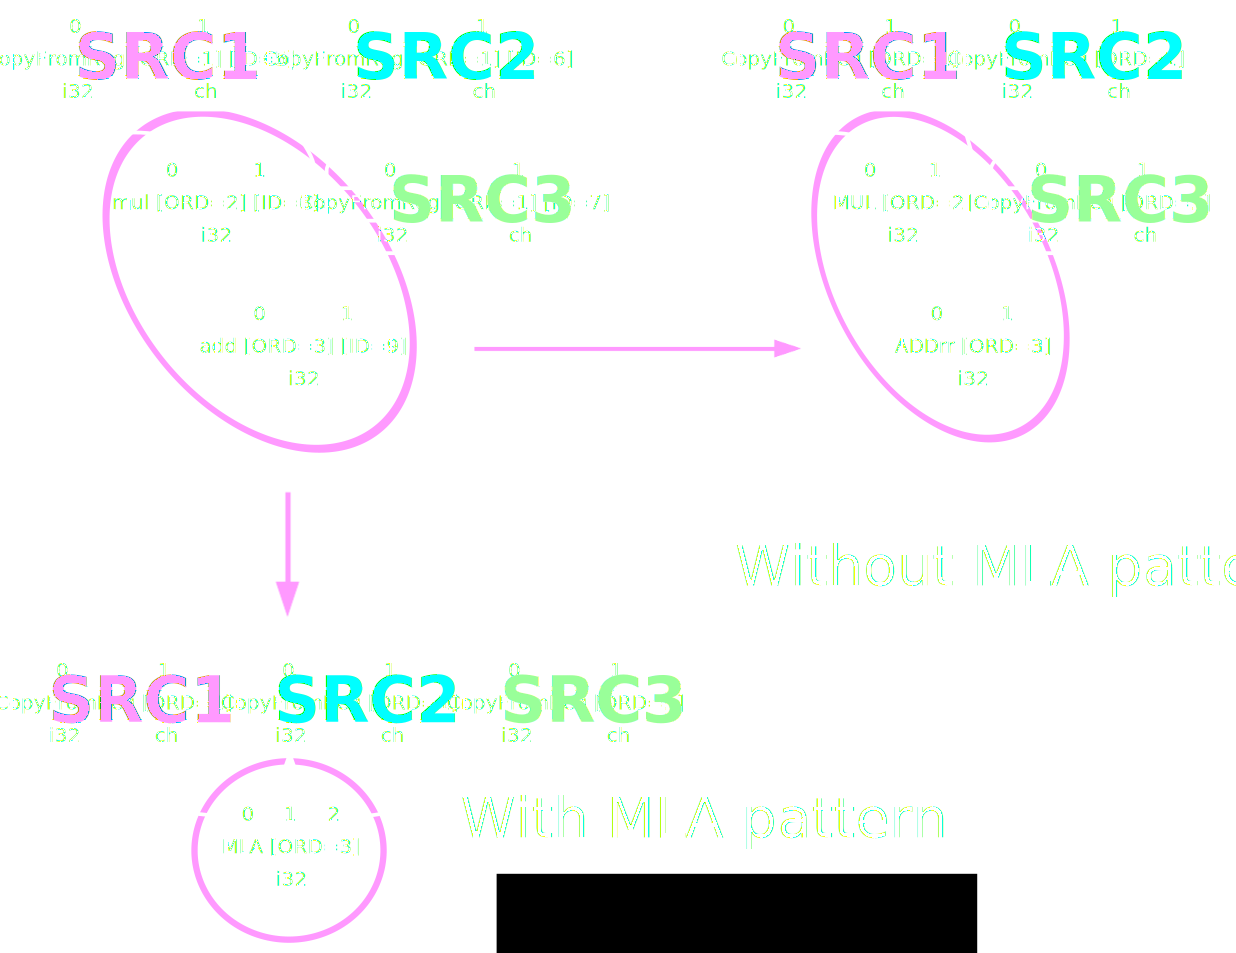
\includegraphics[width = 0.80\textwidth]{examples/ex3/ex3-isel-comparison.pdf}

\end{frame}


\end{document}
